\chapter{Data Experiments}
In this chapter, the parts that compose this project as well as their context are shown. Also, some experiments are demonstrated for comparison with different parameters that could affect this thesis' project's overall accuracy.

\section{Inputs and Outputs}
In previous chapters, it has been specified that this algorithm takes an text input and, according to its contents, a message is shown as an output. The breakdown is as follows.
\subsection{Inputs}
The input that is given is cleaned up and tokenized -- as shown in the previous chapter --, , this is then added to an internal corpus that has weights set for every word in it, effectively working as scores. Every word has a different score in every label, whether it is positive or negative. This score is added up and the highest final score will be the one that the algorithm will detect as the most probable for the text input. However, this has its caveats, small sentences are more likely to be miscategorized because one word can have different applications in the scope of this project, for a more accurate analysis a longer sentence must be written.
\subsection{Outputs}
Depending on the final score, the algorithm will choose a random sentence related to the detected sentiment, this is, as of the time of writing, very rudimentary, but the fact that it is built in Python this can be a building block for a more robust, context-conscious, reply system.
In the training module, however, four extra values are part of the output as well: \textit{Loss}, \textit{Val\_loss}, \textit{Accuracy} and \textit{Val\_accuracy}.
These values are standard in every Neural Network algorithm to observe how poorly the evaluation does within the training dataset, and what the accuracy percentage is, respectively.
The \textit{Val\_} counterparts of these values are the same, but applied to the validation dataset.

\section{Experiments}
In this section, various experiments of this project are shown with varying training data and parameters with the respective accuracy and loss graphs.
The purpose of these experiments is to determine if the parameters chosen for this project are optimal and, if not, correct them and know the reason behind the improvement.
The parameters that could potentially have a great impact on the output of the classification -- and therefore are the best to experiment with -- are the following:
\begin{itemize}
	\item Used datasets: This could influentiate the amount of words in the corpus and have a big impact on how some words are percieved
	\item Training epochs: How many loops does the algorithm go through before being considered fully trained, if this number is too high it could result in \textit{overfitting}, which is, in casual terms, the Neural Network equivalent of overthinking.
	\item Units in the LSTM layer: This unit system, albeit small in the overall scale of things, could make-or-break the algoritm if not tuned correctly.
	\item Categorized sentiments: Reducing the scope of the project could potentially benefit the overall accuracy of the remaining sentiments.
\end{itemize}
The amount of improvement with each experiment is shown with loss and accuracy graphs, which are evaluated every epoch the algorithm is trained. Lower loss and higher accuracy are preferred.
\subsection{Experiment 1}
In this experiment, we look at the base version of this thesis' project.
\begin{table}[!th]
	\caption{Experiment 1's defining characteristics.}
	\vspace{0.5cm}
	\centering
	\begin{tabular}[t]{|l|l|}
	\hline
		Datasets Used & 2: \citet{d1} and \citet{d2}
	\\ \hline
		Epochs & 10
	\\ \hline
		LSTM Layer & 32 units
	\\ \hline
		Categorized Sentiments as ``Bad'' & ``Sadness'', ``Worry'', and ``Fear''.
	\\ \hline	
		 Categorized Sentiments as ``Neutral'' & ``Neutral'' and ``Boredom''.
	\\ \hline	
		Categorized Sentiments as ``Good'' & ``Happiness'', ``Fun'', ``Joy'', and ``Love''.
	\\ \hline
	\end{tabular}
\end{table}

\begin{table}[!bh]
	\caption{Experiment 1's results.}
	\vspace{0.5cm}
	\centering
	\begin{tabular}[t]{|l|l|l|l|}
	\hline
		Loss & 0.6857 & Val\_loss & 0.8499
	\\ \hline
		Accuracy & 0.7151 & Val\_accuracy & 0.6308
	\\ \hline
	\end{tabular}
\end{table}


\begin{figure}[!h]
	\centering
	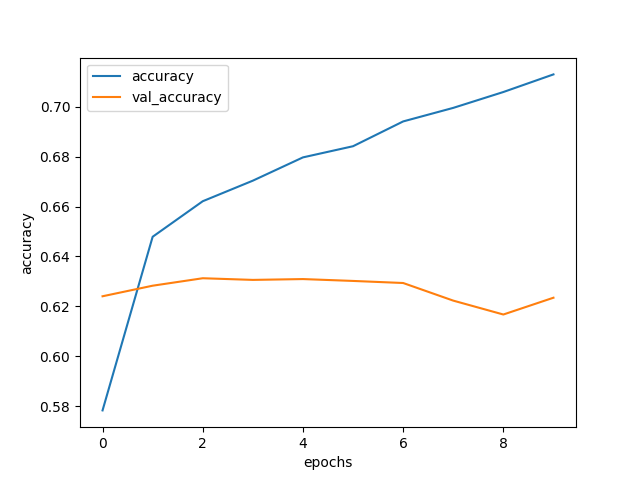
\includegraphics[scale=0.8]{Accuracy_Exp1}
	\caption{Accuracy Graph of Experiment 1}
	\label{fig:accuracy_exp1}
	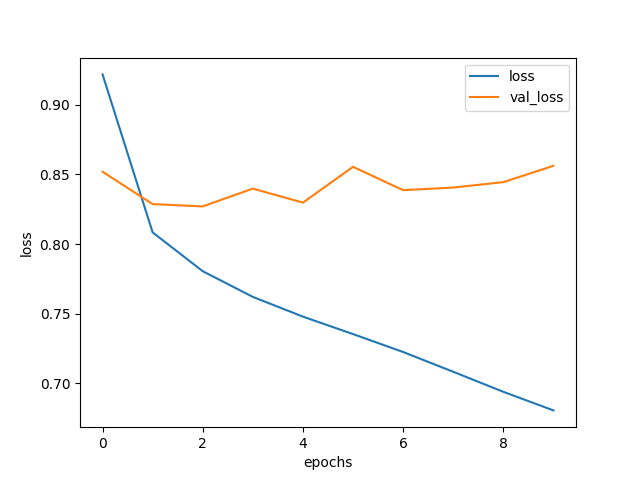
\includegraphics[scale=0.8]{Loss_Exp1}
	\caption{Loss Graph of Experiment 1}
	\label{fig:loss_exp1}
\end{figure}
\pagebreak

\subsection{Experiment 2}
This experiment takes sentences from one more dataset and 3 less categorized sentiments: ``Fear'', ``Joy'', and ``Love''.
\begin{table}[!th]
	\caption{Experiment 2's defining characteristics.}
	\vspace{0.5cm}
	\centering
	\begin{tabular}[t]{|l|l|}
	\hline
		Datasets Used & \makecell{3: \citet{d1}, \citet{d2} and\\ \citet{d3}}
	\\ \hline
		Epochs & 10
	\\ \hline
		LSTM Layer & 32 units
	\\ \hline
		Categorized Sentiments as ``Bad'' & ``Sadness'', and ``Worry''.
	\\ \hline	
		 Categorized Sentiments as ``Neutral'' & ``Neutral'' and ``Boredom''.
	\\ \hline	
		Categorized Sentiments as ``Good'' & ``Happiness'', and ``Fun''.
	\\ \hline
	\end{tabular}
\end{table}

\begin{table}[!bh]
	\caption{Experiment 2's results.}
	\vspace{0.5cm}
	\centering
	\begin{tabular}[t]{|l|l|l|l|}
	\hline
		Loss & 0.5956 & Val\_loss & 0.7649
	\\ \hline
		Accuracy & 0.7576 & Val\_accuracy & 0.6821
	\\ \hline
	\end{tabular}
\end{table}


\begin{figure}[!h]
	\centering
	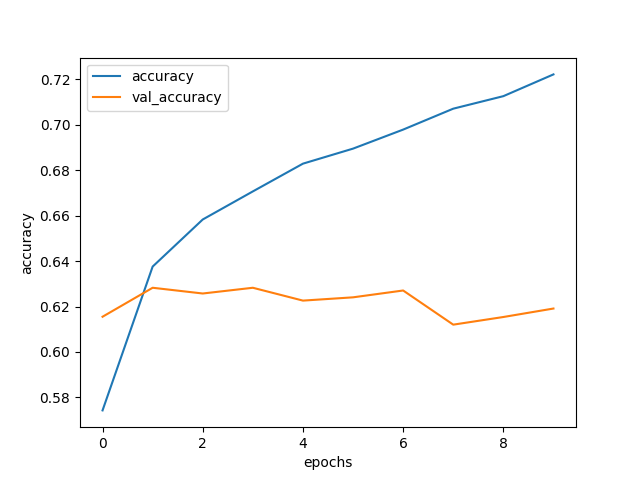
\includegraphics[scale=0.8]{Accuracy_Exp2}
	\caption{Accuracy Graph of Experiment 2}
	\label{fig:accuracy_exp2}
	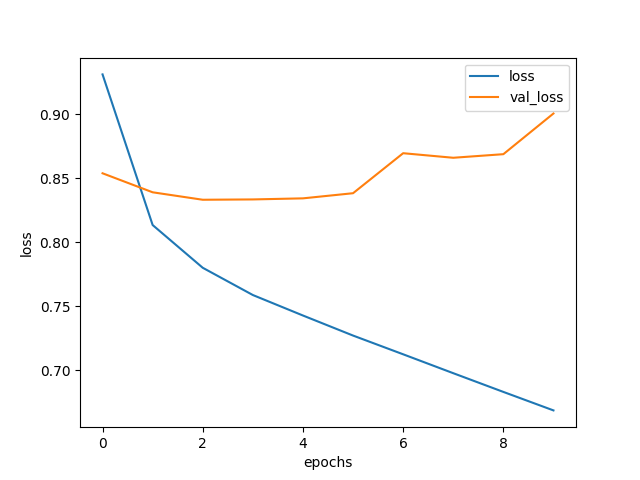
\includegraphics[scale=0.8]{Loss_Exp2}
	\caption{Loss Graph of Experiment 2}
	\label{fig:loss_exp2}
\end{figure}
\pagebreak

\subsection{Experiment 3}
Largely the same as Experiment 2, but the LSTM has more units to work with.
\begin{table}[!th]
	\caption{Experiment 3's defining characteristics.}
	\vspace{0.5cm}
	\centering
	\begin{tabular}[t]{|l|l|}
	\hline
		Datasets Used & \makecell{3: \citet{d1}, \citet{d2} and\\ \citet{d3}}
	\\ \hline
		Epochs & 10
	\\ \hline
		LSTM Layer & 64 units
	\\ \hline
		Categorized Sentiments as ``Bad'' & ``Sadness'', and ``Worry''.
	\\ \hline	
		 Categorized Sentiments as ``Neutral'' & ``Neutral'' and ``Boredom''.
	\\ \hline	
		Categorized Sentiments as ``Good'' & ``Happiness'', and ``Fun''.
	\\ \hline
	\end{tabular}
\end{table}

\begin{table}[!bh]
	\caption{Experiment 3's results.}
	\vspace{0.5cm}
	\centering
	\begin{tabular}[t]{|l|l|l|l|}
	\hline
		Loss & 0.5829 & Val\_loss & 0.7373
	\\ \hline
		Accuracy & 0.7564 & Val\_accuracy & 0.6780
	\\ \hline
	\end{tabular}
\end{table}


\begin{figure}[!h]
	\centering
	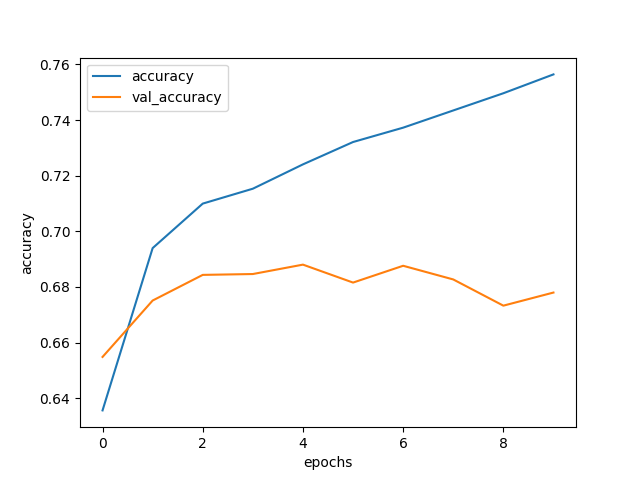
\includegraphics[scale=0.8]{Accuracy_Exp3}
	\caption{Accuracy Graph of Experiment 3}
	\label{fig:accuracy_exp3}
	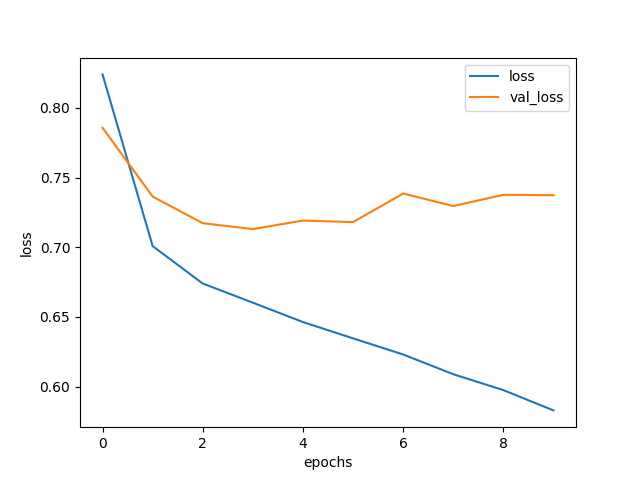
\includegraphics[scale=0.8]{Loss_Exp3}
	\caption{Loss Graph of Experiment 3}
	\label{fig:loss_exp3}
\end{figure}
\pagebreak

\subsection{Experiment 4}
A mix between Experiment 1 and 2. Three datasets with the full sentiment categorization and LSTM with 32 units.
\begin{table}[!h]
	\caption{Experiment 4's defining characteristics.}
	\vspace{0.5cm}
	\centering
	\begin{tabular}[t]{|l|l|}
	\hline
		Datasets Used & \makecell{3: \citet{d1}, \citet{d2} and\\ \citet{d3}}
	\\ \hline
		Epochs & 10
	\\ \hline
		LSTM Layer & 32 units
	\\ \hline
		Categorized Sentiments as ``Bad'' & ``Sadness'', ``Worry'', and ``Fear''.
	\\ \hline	
		 Categorized Sentiments as ``Neutral'' & ``Neutral'' and ``Boredom''.
	\\ \hline	
		Categorized Sentiments as ``Good'' & ``Happiness'', ``Fun'', ``Joy'', and ``Love''.
	\\ \hline
	\end{tabular}
\end{table}

\begin{table}[!b]
	\caption{Experiment 4's results.}
	\vspace{0.5cm}
	\centering
	\begin{tabular}[t]{|l|l|l|l|}
	\hline
		Loss & 0.5455 & Val\_loss & 0.6704
	\\ \hline
		Accuracy & 0.7741 & Val\_accuracy & 0.7210
	\\ \hline
	\end{tabular}
\end{table}


\begin{figure}[!h]
	\centering
	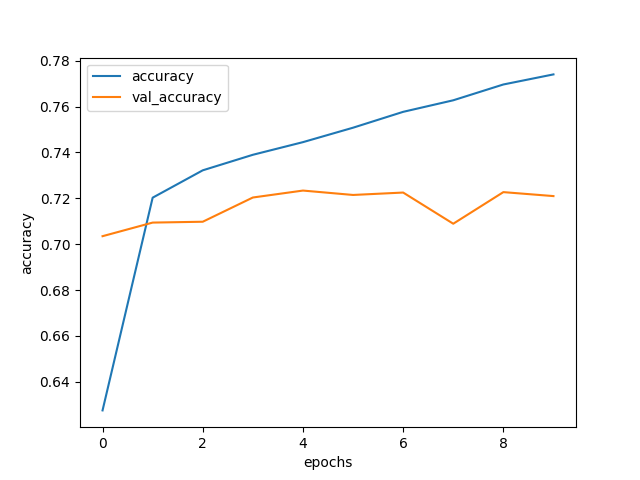
\includegraphics[scale=0.8]{Accuracy_Exp4}
	\caption{Accuracy Graph of Experiment 4}
	\label{fig:accuracy_exp4}
	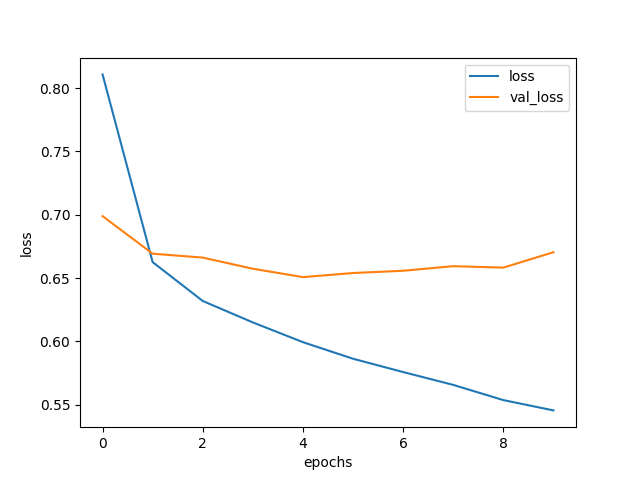
\includegraphics[scale=0.8]{Loss_Exp4}
	\caption{Loss Graph of Experiment 4}
	\label{fig:loss_exp4}
\end{figure}
\pagebreak

\subsection{Experiment 5}
Same as Experiment 4, but with an added dataset with only ``Sadness'' sentences.
\begin{table}[!h]
	\caption{Experiment 5's defining characteristics.}
	\vspace{0.5cm}
	\centering
	\begin{tabular}[t]{|l|l|}
	\hline
		Datasets Used & \makecell{4: \citet{d1}, \citet{d2},\\ \citet{d3}, and \citet{d4}}
	\\ \hline
		Epochs & 10
	\\ \hline
		LSTM Layer & 32 units
	\\ \hline
		Categorized Sentiments as ``Bad'' & ``Sadness'', ``Worry'', and ``Fear''.
	\\ \hline	
		 Categorized Sentiments as ``Neutral'' & ``Neutral'' and ``Boredom''.
	\\ \hline	
		Categorized Sentiments as ``Good'' & ``Happiness'', ``Fun'', ``Joy'', and ``Love''.
	\\ \hline
	\end{tabular}
\end{table}

\begin{table}[!b]
	\caption{Experiment 5's results.}
	\vspace{0.5cm}
	\centering
	\begin{tabular}[t]{|l|l|l|l|}
	\hline
		Loss & 0.5442 & Val\_loss & 0.6620
	\\ \hline
		Accuracy & 0.6620 & Val\_accuracy & 0.7162
	\\ \hline
	\end{tabular}
\end{table}


\begin{figure}[!h]
	\centering
	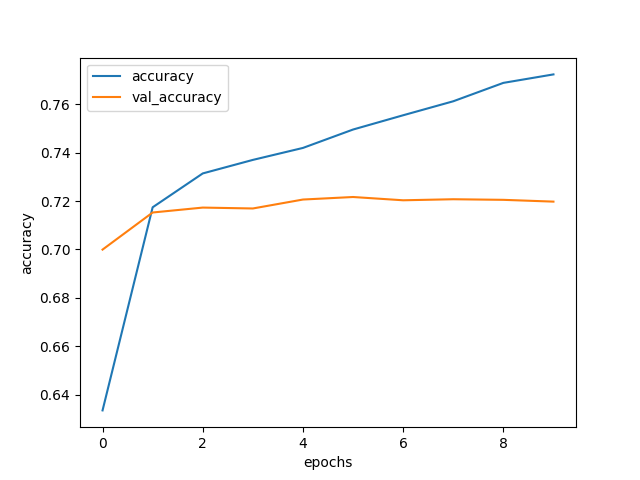
\includegraphics[scale=0.8]{Accuracy_Exp5}
	\caption{Accuracy Graph of Experiment 5}
	\label{fig:accuracy_exp5}
	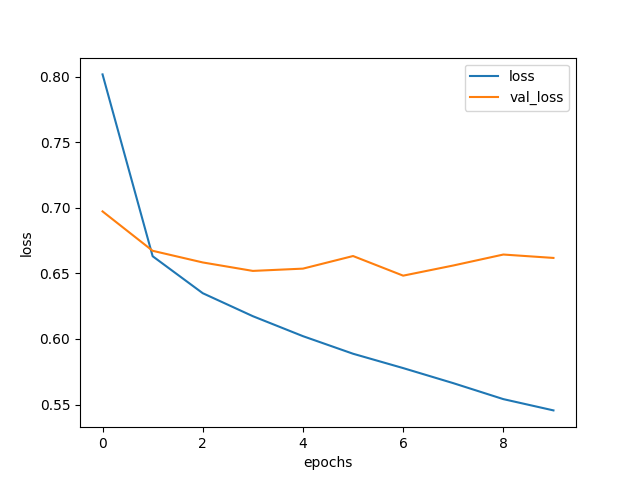
\includegraphics[scale=0.8]{Loss_Exp5}
	\caption{Loss Graph of Experiment 5}
	\label{fig:loss_exp5}
\end{figure}
\pagebreak

\subsection{Experiment 6}
This is the largest change on an experiment, the ``Neutral'' category has been completely disabled with the purpose of seeing how the rest of the data would be classified as.
\begin{table}[!h]
	\caption{Experiment 6's defining characteristics.}
	\vspace{0.5cm}
	\centering
	\begin{tabular}[t]{|l|l|}
	\hline
		Datasets Used & \makecell{4: \citet{d1}, \citet{d2},\\ \citet{d3}, and \citet{d4}}
	\\ \hline
		Epochs & 10
	\\ \hline
		LSTM Layer & 32 units
	\\ \hline
		Categorized Sentiments as ``Bad'' & ``Sadness'', ``Worry'', and ``Fear''.
	\\ \hline	
		 Categorized Sentiments as ``Neutral'' & N/A
	\\ \hline	
		Categorized Sentiments as ``Good'' & ``Happiness'', ``Fun'', ``Joy'', and ``Love''.
	\\ \hline
	\end{tabular}
\end{table}

\begin{table}[!b]
	\caption{Experiment 6's results.}
	\vspace{0.5cm}
	\centering
	\begin{tabular}[t]{|l|l|l|l|}
	\hline
		Loss & 0.6222 & Val\_loss & 0.7186
	\\ \hline
		Accuracy & 0.6550 & Val\_accuracy & 0.5357
	\\ \hline
	\end{tabular}
\end{table}


\begin{figure}[!h]
	\centering
	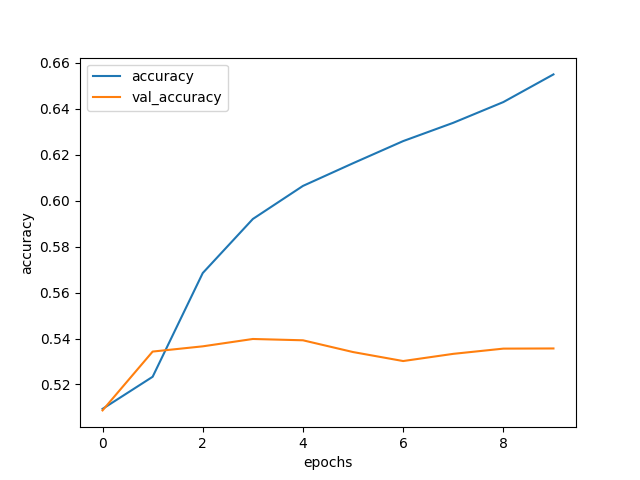
\includegraphics[scale=0.8]{Accuracy_Exp6}
	\caption{Accuracy Graph of Experiment 6}
	\label{fig:accuracy_exp6}
	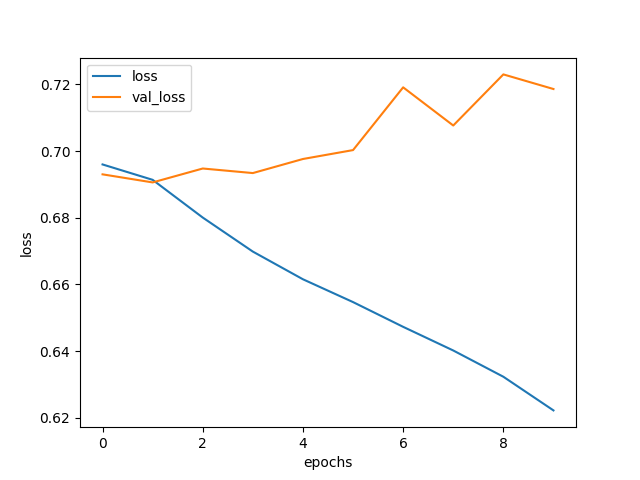
\includegraphics[scale=0.8]{Loss_Exp6}
	\caption{Loss Graph of Experiment 6}
	\label{fig:loss_exp6}
\end{figure}
\pagebreak

\subsection{Experiment 7}
Largely the same as Experiment 5 with half the epochs. This with the purpose of seeing if the data has been overfit.
\begin{table}[!h]
	\caption{Experiment 7's defining characteristics.}
	\vspace{0.5cm}
	\centering
	\begin{tabular}[t]{|l|l|}
	\hline
		Datasets Used & \makecell{4: \citet{d1}, \citet{d2},\\ \citet{d3}, and \citet{d4}}
	\\ \hline
		Epochs & 5
	\\ \hline
		LSTM Layer & 32 units
	\\ \hline
		Categorized Sentiments as ``Bad'' & ``Sadness'', ``Worry'', and ``Fear''.
	\\ \hline	
		 Categorized Sentiments as ``Neutral'' & ``Neutral'' and ``Boredom''.
	\\ \hline	
		Categorized Sentiments as ``Good'' & ``Happiness'', ``Fun'', ``Joy'', and ``Love''.
	\\ \hline
	\end{tabular}
\end{table}

\begin{table}[!b]
	\caption{Experiment 7's results.}
	\vspace{0.5cm}
	\centering
	\begin{tabular}[t]{|l|l|l|l|}
	\hline
		Loss & 0.6041 & Val\_loss & 0.6555
	\\ \hline
		Accuracy & 0.7451 & Val\_accuracy & 0.7197
	\\ \hline
	\end{tabular}
\end{table}


\begin{figure}[!h]
	\centering
	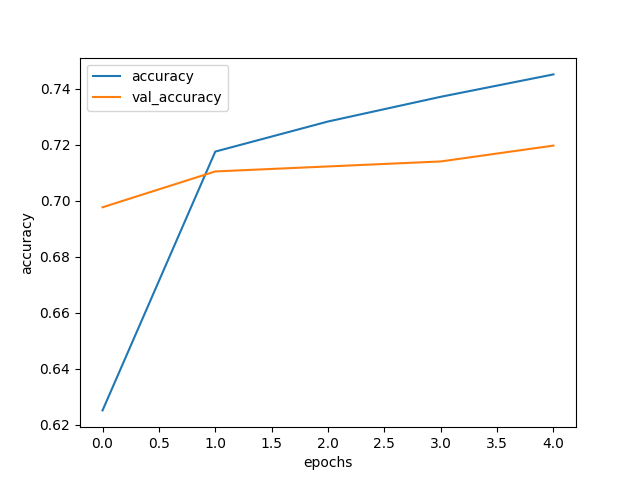
\includegraphics[scale=0.8]{Accuracy_Exp7}
	\caption{Accuracy Graph of Experiment 7}
	\label{fig:accuracy_exp7}
	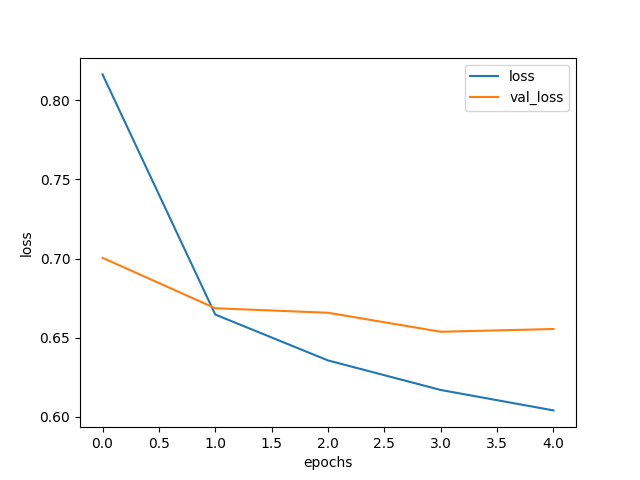
\includegraphics[scale=0.8]{Loss_Exp7}
	\caption{Loss Graph of Experiment 7}
	\label{fig:loss_exp7}
\end{figure}
\pagebreak